%!/usr/bin/env pdflatex
%-*- coding: utf-8 -*-
%@author : Romain Graux
%@date : 2022 May 03, 12:27:08
%@last modified : 2022 June 05, 16:55:15
\label{chapter:sota-pcc}

Numerous methods have been proposed to compress point clouds in the literature. They are usually based on different structures than a classical list of coordinates.                                
Octrees, for example, have been widely used for this purpose \cite{bib:octree}. 
The octree representation consists of diving recursively the three dimensional space as nodes of a tree as shown on Figure \ref{fig:octree}.

\begin{figure}
    \centering
    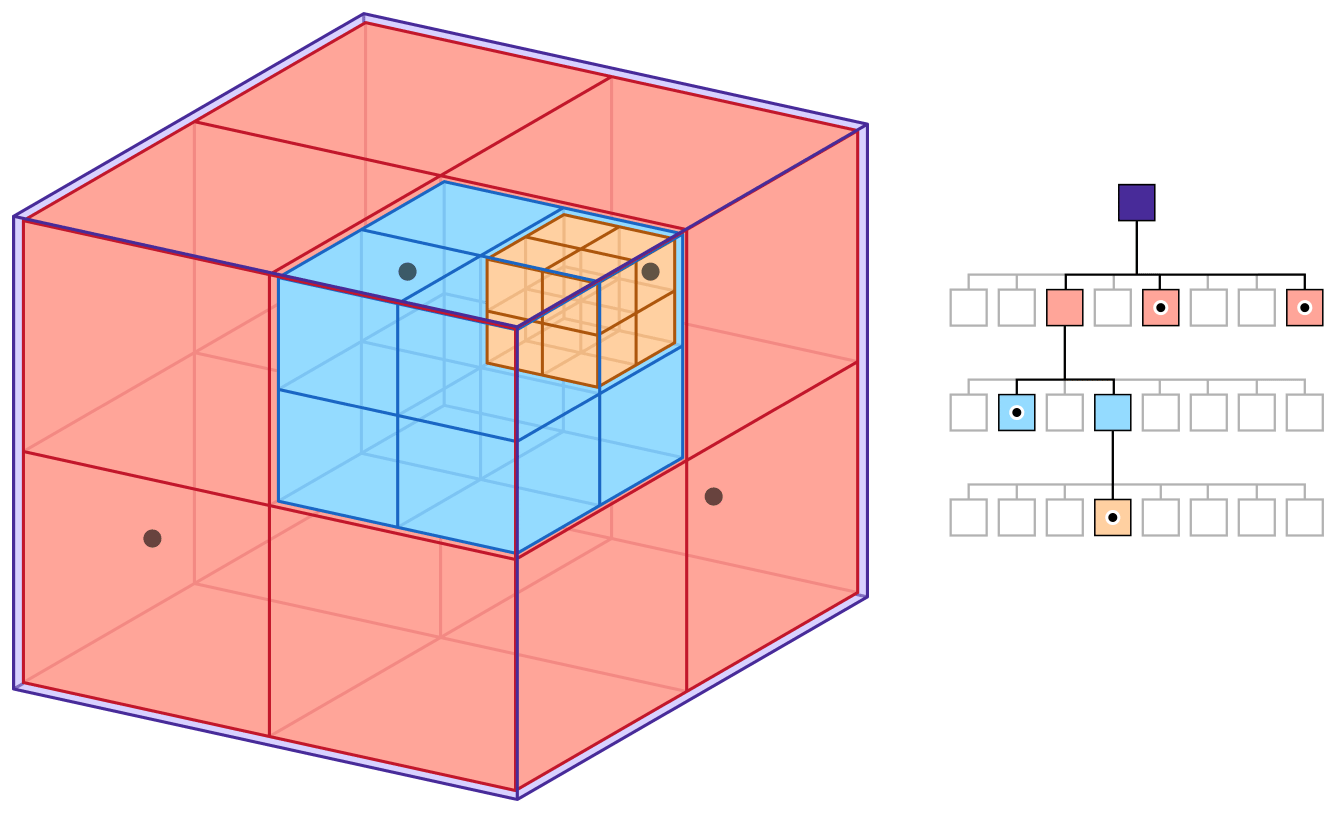
\includegraphics[width=0.6\textwidth]{octree.png}
    \caption{Octree representation of a point cloud}
    \label{fig:octree}
\end{figure}

% \begin{figure}
%     \centering
%     \includegraphics[width=0.6\textwidth]{voxelized.png}
%     \caption{Voxelized representation of a point cloud}
%     \label{fig:voxelized}
% \end{figure}

Compression algorithms using learning based autoencoders architectures have also demonstrated good performance. While some take as input point coordinates \cite{bib:9102866}, others take as input voxelized versions of the point clouds. 
Voxelized point clouds consist of occupancy grid of regular spaced points so that several points are merged together in a single voxel.
A voxel is similar to a three dimensional pixel.
These three dimensional grids can be then used as input for a \textit{3D convolutional layer}.


The current state of the art for point cloud compression that we will use in this project is a model called "Latent Space Slicing For Enhanced Entropy Modeling in Learning-Based Point Cloud Geometry Compression" and that has been developed by Nicolas Frank, Davi Lazzarotto and Touradj Ebrahimi at the MMSPG laboratory (EPFL).

\subsection{Model architecture}

\begin{figure}
    \centering
    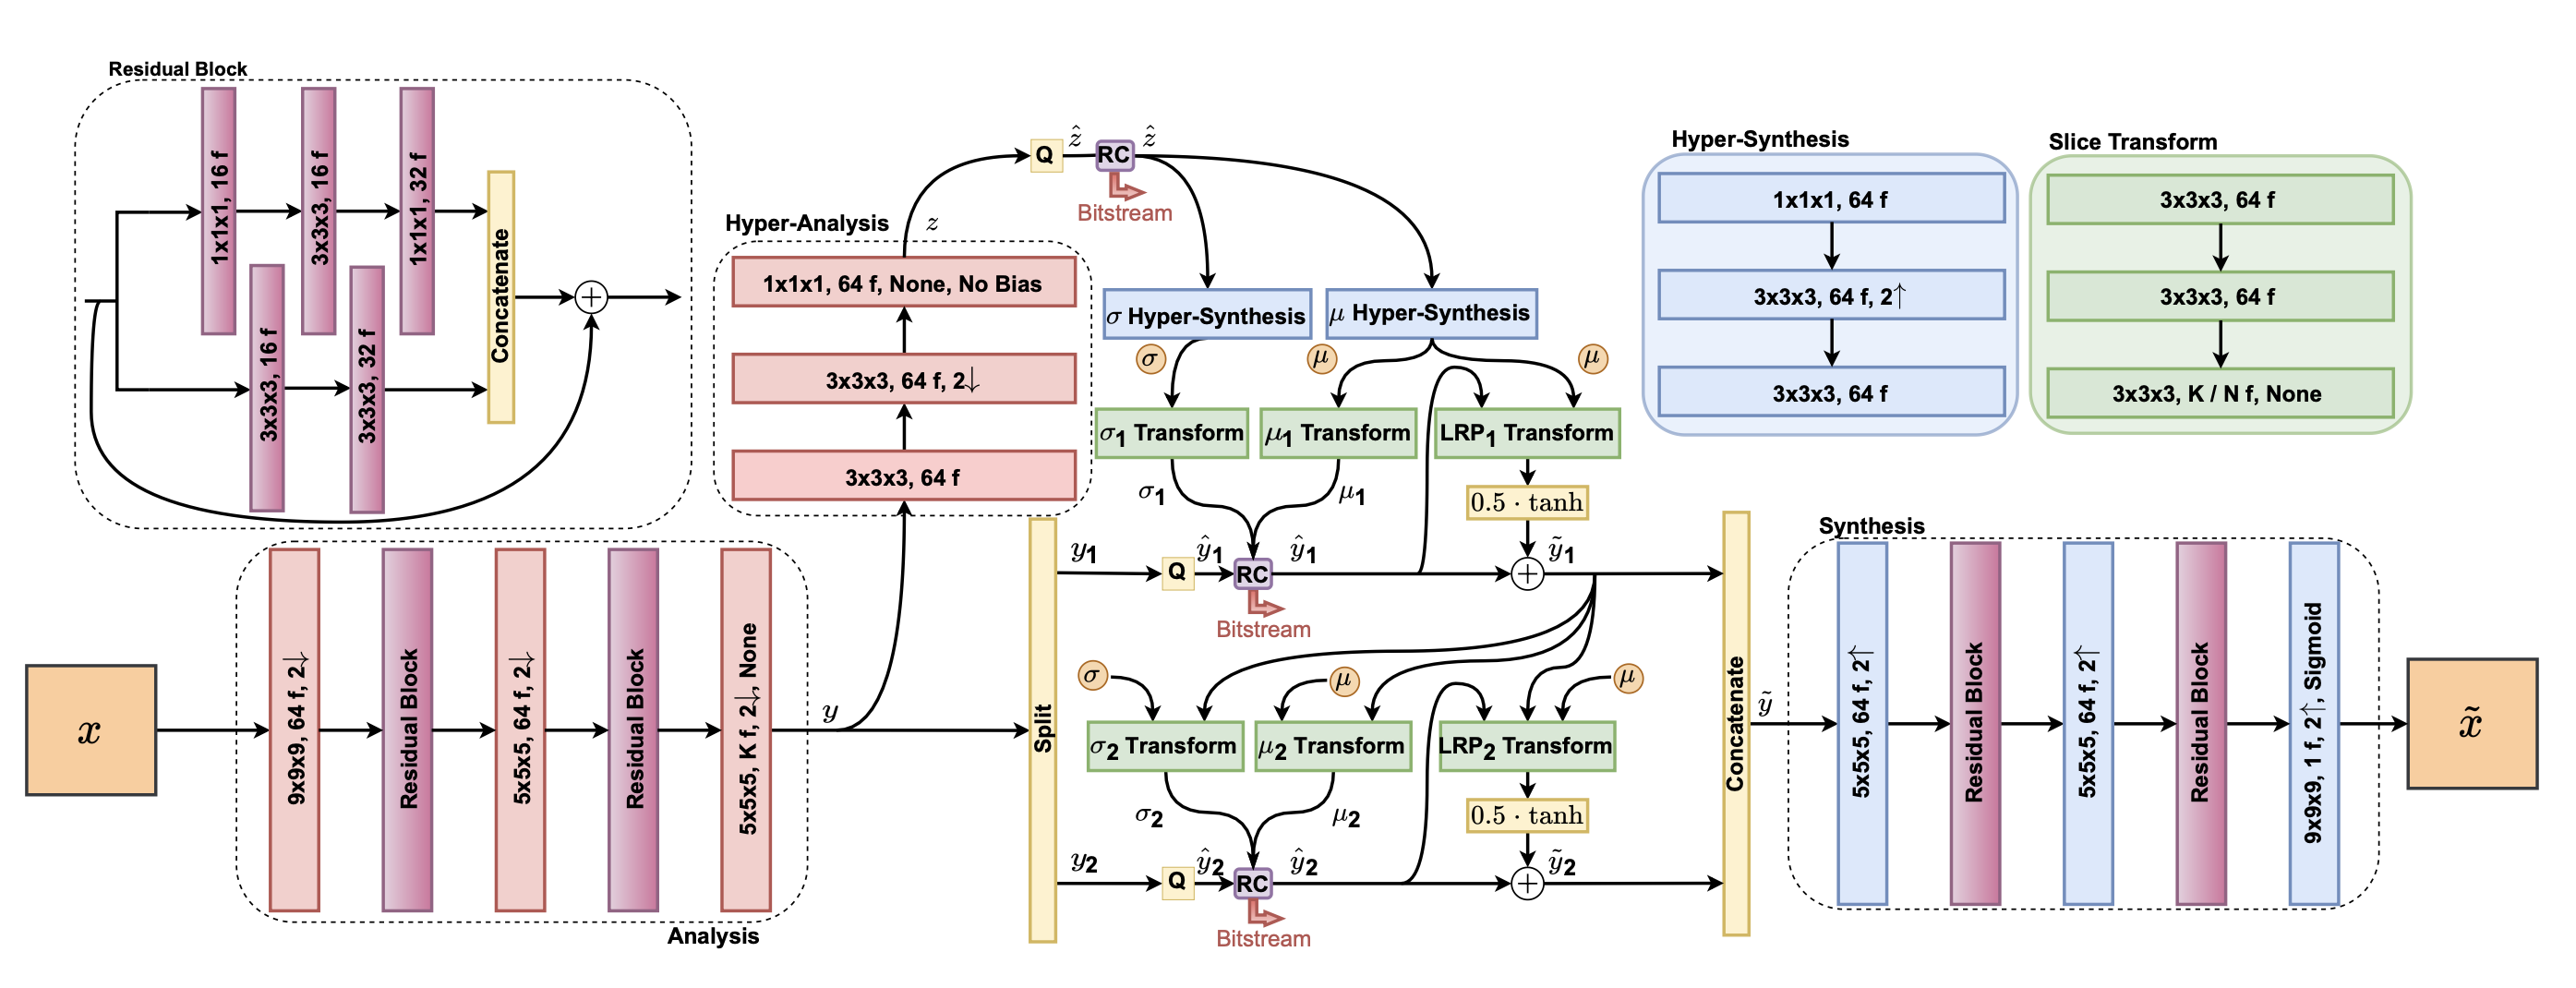
\includegraphics[width=0.8\textwidth]{pcc-geo-slicing-architecture.png}
    \caption{The "Latent Space Slicing For Enhanced Entropy Modeling in Learning-Based Point Cloud Geometry Compression" architecture with $2$ slices.}
    \label{fig:pcc-geo-slicing-architecture}
\end{figure}

This model is shown on Figure \ref{fig:pcc-geo-slicing-architecture} and consists in a 3D autoencoder architecture with latent entropy coding. 
The input of the model is an occupancy cubic grid with $k \times k \times k$ voxels represented by $1$ when occupied and $0$ otherwise. 


The first block (Analysis transform) of the model is composed of 3 \textit{3D convolutional layers} and 2 \textit{convolutional residual blocks} arranged staggered which produces a latent representation $y$ of shape $l \times l \times l \times d$ with $d$ being the latent dimension. 


This latent representation is then fed into an Hyper-Analysis transform block yielding $z$. This hyperprior is passed to the bitstream as side information after quantization, and is used to model the entropy of the quantized latent features $\hat{y}$ after going through the hyper-synthesis. 

While in other solutions for learning-based point cloud compression the hyperprior would be the only variable used to estimate the scale and mean of $\hat{y}$, they use previously decoded channels for entropy modeling.

The latent representation $y$ is sliced along the channel dimension into $N$ non-overlapping and equally sized tensors $y_i$ with $i \in \{1, \dots, N\}$. 

Once the latent representation $y$ is sliced, they compute the entropy parameters ($\mu_i,\,\sigma_i$) for each slice $y_i$ from the global entropy parameters ($\mu,\,\sigma$) and the previously decoded latent representation slices $\tilde{y}_j\,\forall j \in \{0,\dots,i-1\}$. 

The final latent representation reconstruction $\tilde{y}_i$ is produced from $\hat{y}_i$ after going through a latent residual prediction (LRP) transform that predicts the quantization error $y_i - \hat{y}_i$ in order to take into account this error from the global entropy parameters ($\mu,\,\sigma$), the current $\hat{y}_i$ and previously decoded latent representation slices $\tilde{y}_j\,\forall j \in \{0,\dots,i\}$. A \textit{tanh} non-linearity scaled by a factor $0.5$ is applied to the output of the transform to keep the output of the LRP within the range of quantization error. 
The predicted residuals are then added to $\hat{y}_i$, generating $\tilde{y}_i$.
These slices are then concatenated along the channel dimension before going through the synthesis transform. This last learned block finally generates the output block $\tilde{x}$ containing a probability estimation for the occupancy of each voxel in the grid.

They trained the model from end-to-end between the input occupancy grid and output probability occupancy grid as a rate-distortion minimization problem represented by the loss function expressed as $\mathcal{L} = R + \lambda D$. The trade-off parameter $\lambda$ is used to balance the importance of compression rate against reconstruction quality. 
The distortion is computed from a focal loss (FL) which can be expressed as: 
$$
\text{FL}(x, \tilde{x}) = -x \alpha (1-\tilde{x})^{\gamma} \text{log}(\tilde{x}) - (1-x) (1-\alpha) \tilde{x}^{\gamma} \text{log}(1-\tilde{x})
$$

\noindent with $\alpha$ and $\gamma$ being configurable hyperparameters. This focal loss is a so-called \href{https://www.tensorflow.org/api_docs/python/tf/keras/losses/BinaryFocalCrossentropy}{binary weighted focal crossentropy loss}.

The last step to recover the actual binary occupancy grid from the output probability occupancy grid $\tilde{x}$ is to apply a threshold $t$ and round every value above $t$ to $1$ and $0$ otherwise. While a naive approach would be to set this threshold $t$ to $0.5$, they decided to find the best threshold $t \in [0,1]$ such that it minimizes the point-to-point MSE between the original and reconstructed rounded block.
